% -*- latex -*-
%%%%%%%%%%%%%%%%%%%%%%%%%%%%%%%%%%%%%%%%%%%%%%%%%%%%%%%%%%%%%%%%
%%%%
%%%% This TeX file is part of the course
%%%% Introduction to Scientific Programming in C++/Fortran2003
%%%% copyright 2019-2021 Victor Eijkhout eijkhout@tacc.utexas.edu
%%%%
%%%% amazon.tex : exercises for delivery trucks
%%%%
%%%%%%%%%%%%%%%%%%%%%%%%%%%%%%%%%%%%%%%%%%%%%%%%%%%%%%%%%%%%%%%%

This section contains a sequence of exercises that builds up to a
simulation of delivery truck scheduling.

\Level 0 {Problem statement}

Scheduling the route of a delivery truck is a well-studied
problem. For instance, minimizing the total distance that the truck
has to travel corresponds to the \indexacdef{TSP}. However, in the
case of \indextermbus{Amazon}{delivery truck} scheduling the problem
has some new aspects:
\begin{itemize}
\item A customer is promised a window of days when delivery can take
  place. Thus, the truck can split the list of places into sublists,
  with a shorter total distance than going through the list in one
  sweep.
\item Except that \indextermbus{Amazon}{prime} customers need their
  deliveries guaranteed the next day.
\end{itemize}

\Level 0 {Coding up the basics}

Before we try finding the best route, let's put the basics in place
to have any sort of route at all.

\Level 1 {Address list}

You probably need a class \lstinline{Address} that describes the
location of a house where a delivery has to be made.
\begin{itemize}
\item
  For simplicity, let give a house $(i,j)$ coordinates.
\item We probably need a \lstinline{distance} function between two
  addresses. We can either assume
  that we can travel in a straight line between two houses, or that
  the city is build on a grid, and you can apply the so-called
  \indexterm{Manhattan distance}.
\item The address may also require a field recording the last possible
  delivery date.
\end{itemize}

\begin{exercise}
  Code a class \lstinline{Address} with the above functionality, and
  test it.
  \snippetwithoutput{amazonaddressuse}{amazon}{address}
\end{exercise}

Next we need a class \lstinline{AddressList} that contains a list of
addresses.

\begin{exercise}
  Implement a class \lstinline{AddressList}; it probably needs the
  following methods:
  \begin{itemize}
  \item \lstinline{add_address} for constructing the list;
  \item \lstinline{length} to give the distance one has to travel to
    visit all addresses in order;
  \item \lstinline{index_closest_to} that gives you the address on the
    list closests to another address, presumably not on the list.
  \end{itemize}
\end{exercise}

\Level 1 {Add a depot}

Next, we model the fact that the route
needs to start and end at the depot, which we put arbitrarily at
coordinates~$(0,0)$. We could construct an \lstinline{AddressList}
that has the depot as first and last element, but that may run into
problems:
\begin{itemize}
\item If we reorder the list to minimize the driving distance, the
  first and last elements may not stay in place.
\item We may want elements of a list to be unique: having an address
  twice means two deliveries at the same address, so the
  \lstinline{add_address} method would check that an address is not
  already in the list.
\end{itemize}
We can solve this by making a class \lstinline{Route}, which inherits
from \lstinline{AddressList}, but the methods of which leave the first
and last element of the list in place.

\Level 1 {Greedy construction of a route}

\index{greedy search|see{search, greedy}}
%
Next we need to construct a route. Rather than solving the full
\ac{TSP}, we start by employing a \indextermsubdef{greedy}{search} strategy:
\begin{quote}
  Given a point, find the next point by some local optimality test,
  such as shortest distance. Never look back to revisit the route you
  have constructed so far.
\end{quote}
Such a strategy is likely to give an improvement, but most likely will
not give the optimal route.

Let's write a method
\begin{lstlisting}
Route::Route greedy_route();
\end{lstlisting}
that constructs a new address list, containing the same addresses, but
arranged to give a shorter length to travel.

\begin{exercise}
  Write the \lstinline{greedy_route} method for the
  \lstinline{AddressList} class.
  \begin{enumerate}
  \item Assume that the route starts at the depot, which is located
    at~$(0,0)$. Then  incrementally construct a new list by:
    \item Maintain an \lstinline{Address} variable
      \lstinline{we_are_here} of the current location;
    \item repeatedly find the address closest to \lstinline{we_are_here}.
  \end{enumerate}
  Extend this to a method for the
  \lstinline{Route} class by working on the subvector that does not
  contain the final element.

  Test it on this example:
  \answerwithoutput{square5}{amazon}{square5}
\end{exercise}

Reorganizing a list can be done in a number of ways.
\begin{itemize}
\item First of all, you can try to make the changes in place. This
  runs into the objection that maybe you want to save the original
  list; also, while swapping two elements can be done with the
  \lstinline{insert} and \lstinline{erase} methods, more complicated
  operations are tricky.
\item Alternatively, you can incrementally construct a new list. Now
  the main problem is to keep track of which elements of the original
  have been processed. You could do this by giving each adress a
  boolean field \lstinline{done}, but you could also make a copy of
  the input list, and remove the elements that have been processed.
  For this, study the \lstinline{erase} method for \lstinline{vector} objects.
\end{itemize}

\Level 0 {Optimizing the route}

The above suggestion of each time finding the closest address is known
as a \indextermsub{greedy}{search} strategy. It does not give you
the optimal solution of the \ac{TSP}. Finding the optimal solution of
the \ac{TSP} is hard to program --~you could do it recursively~-- and
takes a lot of time as the number of addresses grows. In fact, the
\ac{TSP} is probably the most famous of the class of
\indexterm{NP-hard} problems, which are generally believed to have a
running time that grows faster than polynomial in the problem size.

\begin{figure}[ht]
  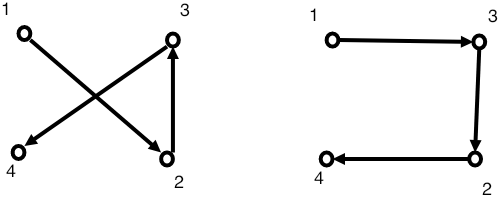
\includegraphics[scale=.4]{opt2}
  \caption{Illustration of the `opt2' idea of reversing part of a
    path}
  \label{fig:opt2}
\end{figure}

However, you can approximate the solution heuristically. One method,
the Kernighan-Lin algorithm~\cite{KL:TSP}, is based on the
\indexterm{opt2} idea: if you have a path that `crosses itself', you
can make it shorter by reversing part of it. Figure~\textbookref{fig:opt2}
shows that the path $1--2--3--4$ can be made shorter by reversing part
of it, giving $1--3--2--4$. Since recognizing where a path crosses
itself can be hard, or even impossible for graphs that don't have
Cartesian coordinates associated, we adopt a scheme:
\begin{verbatim}
for all nodes m<n on the path [1..N]:
  make a new route from
    [1..m-1] + [m--n].reversed + [n+1..N]
  if the new route is shorter, keep it
\end{verbatim}

\begin{exercise}
  Code the opt2 heuristic: write a method to reverse part of the
  route, and write the loop that tries this with multiple starting and
  ending points. Try it out on some simple test cases to convince you
  that your code works as intended.
\end{exercise}

\begin{exercise}
  What is the runtime complexity of this heuristic solution?
\end{exercise}

\begin{exercise}
  Earlier you had programmed the greedy heuristic. Compare the
  improvement you get from the opt2 heuristic, starting both with the
  given list of addresses, and with a greedy traversal of it.
\end{exercise}

\Level 0 {Multiple trucks}
\label{sec:amazon-days}

If we introduce multiple delivery trucks, we get the `Multiple
Traveling Salesman Problem'~\cite{Bektas:MTSP}.
With this we can module both the cases of multiple trucks being out on
delivery on the same day, or one truck spreading deliveries over
multiple days. For now we don't distinguish between the two.

The first question is how to divide up the addresses.
\begin{enumerate}
\item We could split the list in two, using some geometric test. This
  is a good model for the case where multiple trucks are out on the
  same day. However, if we use this as a model for the same truck
  being out on multiple days, we are missing the fact that new
  addresses can be added on the first day, messing up the neatly
  separated routes.
\item Thus it may in fact be reasonable to assume that all trucks get
  an essentially random list of addresses.
\end{enumerate}

\begin{figure}[ht]
  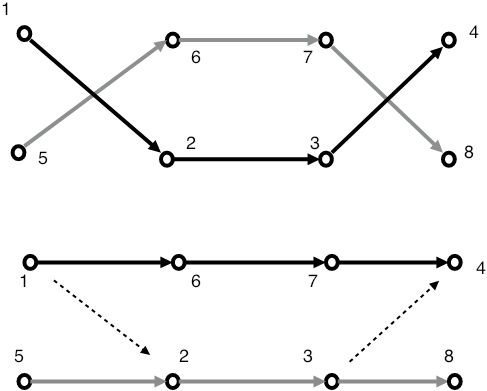
\includegraphics[scale=.6]{opt2_lr}
  \caption{Extending the `opt2' idea to multiple paths}
  \label{fig:opt2_lr}
\end{figure}

Can we extend the opt2 heuristic to the case of multiple paths?
For inspiration take a look at figure~\textbookref{fig:opt2_lr}: instead of
modifying one path, we could switch bits out bits between one path and another.
When you write the code, take into account that the other path may be
running backwards! This means that based on split points in the first
and second path you know have four resulting modified paths to
consider.

\begin{figure}[ht]
  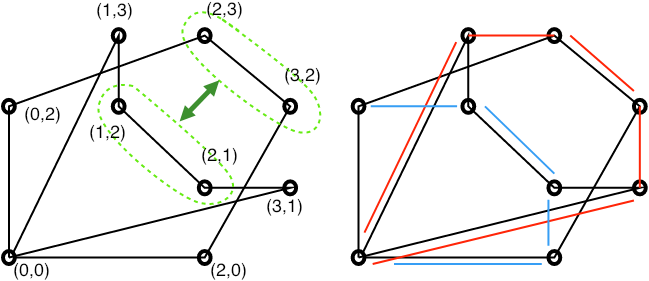
\includegraphics[scale=.6]{tsp2-example}
  \caption{Multiple paths test case}
  \label{fig:tsp2-example}
\end{figure}

\begin{exercise}
  Write a function that optimizes two paths simultaneously using the
  multi-path version of the opt2 heuristic. For a test case, see
  figure~\textbookref{fig:tsp2-example}.

  You have quite a bit of freedom here:
  \begin{itemize}
  \item The start points of the two segments should be chosen independently;
  \item the lengths can be chosen independently, but need not; and finally
  \item each segment can be reversed.
  \end{itemize}
  More flexibility also means a longer runtime of your program.
  Does it pay off? Do some tests and report results.
\end{exercise}

Based on the above description there will be a lot of code
duplication. Make sure to introduce functions and methods for various
operations.

\Level 0 {Amazon prime}

In section~\textbookref{sec:amazon-days} you made the assumption that it
doesn't matter on what day a package is delivered. This changes with
\indextermbus{Amazon}{prime}, where a package has to be delivered
guaranteed on the next day.

\begin{exercise}
  Explore a scenario where there are two trucks, and each have a number
  of addresses that can not be exchanged with the other route.
  How much longer is the total distance? Experiment with
  the ratio of prime to non-prime addresses.
\end{exercise}

\Level 0 {Dynamicism}

So far we have assumed that the list of addresses to be delivered to
is given. This is of course not true: new deliveries will need to be
scheduled continuously.

\begin{exercise}
  Implement a scenario where every day a random number of new
  deliveries is added to the list. Explore strategies and design choices.
\end{exercise}

\Level 0 {Ethics}

People sometimes criticize Amazon's labor policies,
including regarding its drivers.
Can you make any observations from your simulations in this respect?
